\documentclass[a4paper,11pt]{article}
\input{/home/tof/Documents/Cozy/latex-include/preambule_doc.tex}
\input{/home/tof/Documents/Cozy/latex-include/preambule_commun.tex}
\newcommand{\showprof}{show them}  % comment this line if you don't want to see todo environment
\setlength{\fboxrule}{0.8pt}
\fancyhead[L]{\fbox{\Large{\textbf{RecTex 01}}}}
\fancyhead[C]{\textbf{Recherche textuelle}}
\newdate{madate}{10}{09}{2020}
%\fancyhead[R]{\displaydate{madate}} %\today
%\fancyhead[R]{Seconde - SNT}
%\fancyhead[R]{Première - NSI}
\fancyhead[R]{Terminale - NSI}
\fancyfoot[L]{\vspace{1mm}Christophe Viroulaud}
\AtEndDocument{\label{lastpage}}
\fancyfoot[C]{\textbf{Page \thepage/\pageref{lastpage}}}
\fancyfoot[R]{\includegraphics[width=2cm,align=t]{/home/tof/Documents/Cozy/latex-include/cc.png}}
\usepackage{tikz}

\begin{document}
\section{Problématique}
Rechercher les occurrences d'un mot dans un texte est une fonctionnalité intégrée dans tous les logiciels de traitements de texte. Si la tâche semble aisée dans un texte d'une seule page, nous pouvons nous interroger sur l'efficacité de la recherche d'un mot dans un livre entier.
%également dans EDI
\begin{center}
    \framebox{Comment effectuer une recherche textuelle efficace?}
\end{center}
\section{Approche naïve}
\subsection{Principe}
La première méthode à laquelle nous pouvons penser consiste à:
\begin{itemize}
    \item observer une \textbf{fenêtre} du texte,
    \item dans cette fenêtre, comparer chaque lettre du \textbf{motif} recherché au texte,
    \item décaler la fenêtre d'un cran dès qu'il n'y a pas de correspondance.
\end{itemize}
\begin{center}
    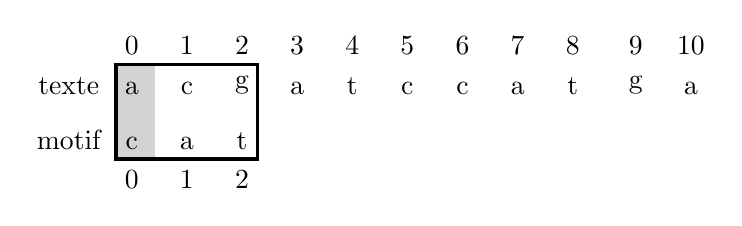
\begin{tikzpicture}
        \fill[LightGray] (1.9,0.5)--(2.4,0.5) -- (2.4,-0.7) -- (1.9,-0.7) -- cycle;
        \foreach \a/\b in {2.1/0,2.8/1,3.5/2,4.2/3,4.9/4,5.6/5,6.3/6,7/7,7.7/8,8.5/9,9.2/10}
            {\node[anchor=south] at (\a,0.5) {\b};}
        \node[anchor=south] at(1.3,0){texte};
        \foreach \a/\b in {2.1/a,2.8/c,3.5/g,4.2/a,4.9/t,5.6/c,6.3/c,7/a,7.7/t,8.5/g,9.2/a}
            {\node[anchor=south] at (\a,0) {\b};}

        \node[anchor=south] at(1.3,-0.7){motif};
        \foreach \a/\b in {2.1/c,2.8/a,3.5/t}
            {\node[anchor=south] at (\a,-0.7) {\b};}
        \foreach \a/\b in {2.1/0,2.8/1,3.5/2}
            {\node[anchor=south] at (\a,-1.2) {\b};}
        \draw[very thick] (1.9,0.5)--(3.7,0.5) -- (3.7,-0.7) -- (1.9,-0.7) -- cycle;
    \end{tikzpicture}
    \captionof{figure}{Première comparaison: pas de correspondance}
\end{center}
\begin{center}
    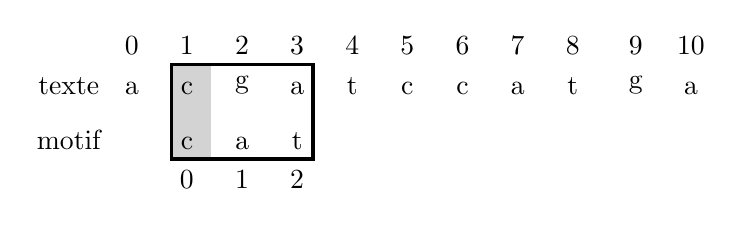
\begin{tikzpicture}
        \fill[LightGray] (2.6,0.5)--(3.1,0.5) -- (3.1,-0.7) -- (2.6,-0.7) -- cycle;
        \foreach \a/\b in {2.1/0,2.8/1,3.5/2,4.2/3,4.9/4,5.6/5,6.3/6,7/7,7.7/8,8.5/9,9.2/10}
            {\node[anchor=south] at (\a,0.5) {\b};}
        \node[anchor=south] at(1.3,0){texte};
        \foreach \a/\b in {2.1/a,2.8/c,3.5/g,4.2/a,4.9/t,5.6/c,6.3/c,7/a,7.7/t,8.5/g,9.2/a}
            {\node[anchor=south] at (\a,0) {\b};}

        \node[anchor=south] at(1.3,-0.7){motif};
        \foreach \a/\b in {2.8/c,3.5/a,4.2/t}
            {\node[anchor=south] at (\a,-0.7) {\b};}
        \foreach \a/\b in {2.8/0,3.5/1,4.2/2}
            {\node[anchor=south] at (\a,-1.2) {\b};}
        \draw[very thick] (2.6,0.5)--(4.4,0.5) -- (4.4,-0.7) -- (2.6,-0.7) -- cycle;
    \end{tikzpicture}
    \captionof{figure}{Première comparaison: correspondance}
\end{center}
\begin{center}
    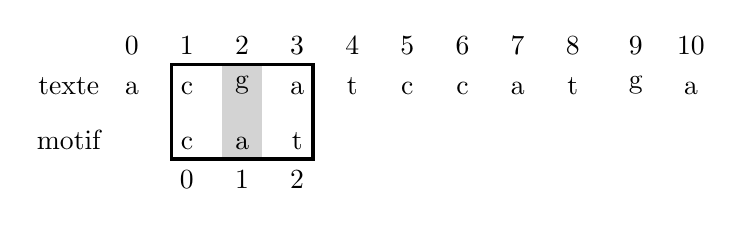
\begin{tikzpicture}
        \fill[LightGray] (3.25,0.5)--(3.75,0.5) -- (3.75,-0.7) -- (3.25,-0.7) -- cycle;
        \foreach \a/\b in {2.1/0,2.8/1,3.5/2,4.2/3,4.9/4,5.6/5,6.3/6,7/7,7.7/8,8.5/9,9.2/10}
            {\node[anchor=south] at (\a,0.5) {\b};}
        \node[anchor=south] at(1.3,0){texte};
        \foreach \a/\b in {2.1/a,2.8/c,3.5/g,4.2/a,4.9/t,5.6/c,6.3/c,7/a,7.7/t,8.5/g,9.2/a}
            {\node[anchor=south] at (\a,0) {\b};}

        \node[anchor=south] at(1.3,-0.7){motif};
        \foreach \a/\b in {2.8/c,3.5/a,4.2/t}
            {\node[anchor=south] at (\a,-0.7) {\b};}
        \foreach \a/\b in {2.8/0,3.5/1,4.2/2}
            {\node[anchor=south] at (\a,-1.2) {\b};}
        \draw[very thick] (2.6,0.5)--(4.4,0.5) -- (4.4,-0.7) -- (2.6,-0.7) -- cycle;
    \end{tikzpicture}
    \captionof{figure}{Deuxième comparaison: pas de correspondance}
\end{center}
\subsection{Implémentation}
\begin{activite}
    \begin{enumerate}
        \item Écrire la fonction \textbf{\texttt{recherche\_naive(texte: str, motif: str) $\rightarrow$ int}} qui renvoie la position du \emph{motif} dans le \emph{texte} ou -1 s'il n'est pas présent.
        \item Estimer la complexité temporelle de cet algorithme dans le pire des cas: le motif n'est pas présent dans le texte.
    \end{enumerate}
\end{activite}
\section{Approche plus efficace: Boyer-Moore}
%dvp en 1977
\subsection{Recherche à l'envers}
La première idée de cet algorithme est de commencer la recherche \textbf{en partant de la fin du motif}.
% on parcourt toujours la chaîne de gauche à droite
\begin{center}
    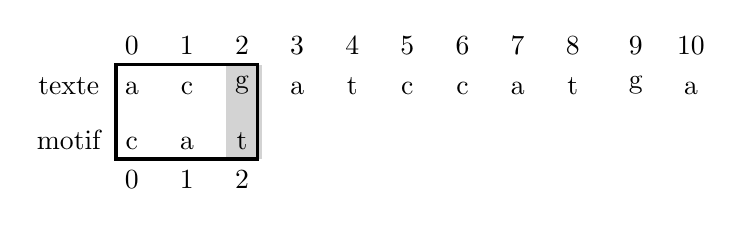
\begin{tikzpicture}
        \fill[LightGray] (3.3,0.5)--(3.75,0.5) -- (3.75,-0.7) -- (3.3,-0.7) -- cycle;
        \foreach \a/\b in {2.1/0,2.8/1,3.5/2,4.2/3,4.9/4,5.6/5,6.3/6,7/7,7.7/8,8.5/9,9.2/10}
            {\node[anchor=south] at (\a,0.5) {\b};}
        \node[anchor=south] at(1.3,0){texte};
        \foreach \a/\b in {2.1/a,2.8/c,3.5/g,4.2/a,4.9/t,5.6/c,6.3/c,7/a,7.7/t,8.5/g,9.2/a}
            {\node[anchor=south] at (\a,0) {\b};}

        \node[anchor=south] at(1.3,-0.7){motif};
        \foreach \a/\b in {2.1/c,2.8/a,3.5/t}
            {\node[anchor=south] at (\a,-0.7) {\b};}
        \foreach \a/\b in {2.1/0,2.8/1,3.5/2}
            {\node[anchor=south] at (\a,-1.2) {\b};}
        \draw[very thick] (1.9,0.5)--(3.7,0.5) -- (3.7,-0.7) -- (1.9,-0.7) -- cycle;
    \end{tikzpicture}
    \captionof{figure}{Première comparaison: pas de correspondance}
    \label{depart}
\end{center}
Pour l'instant cette approche ne semble par apporter d'amélioration par rapport à l'algorithme précédent.
\subsection{Décalages par sauts}
Si on s'intéresse au motif, on peut remarquer qu'il ne contient pas la lettre \textbf{g} (la dernière lettre de la fenêtre). Les comparaisons \ref{inutile1} et \ref{inutile2} sont donc inutiles.
\begin{center}
    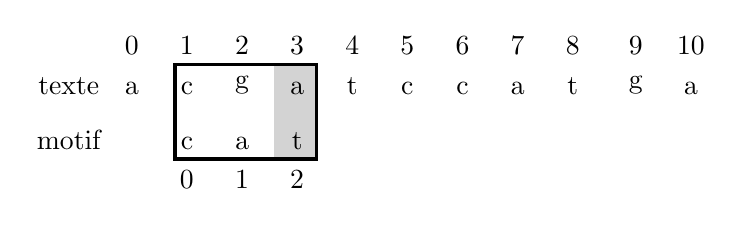
\begin{tikzpicture}
        \fill[LightGray] (3.9,0.5)--(4.45,0.5) -- (4.45,-0.7) -- (3.9,-0.7) -- cycle;
        \foreach \a/\b in {2.1/0,2.8/1,3.5/2,4.2/3,4.9/4,5.6/5,6.3/6,7/7,7.7/8,8.5/9,9.2/10}
            {\node[anchor=south] at (\a,0.5) {\b};}
        \node[anchor=south] at(1.3,0){texte};
        \foreach \a/\b in {2.1/a,2.8/c,3.5/g,4.2/a,4.9/t,5.6/c,6.3/c,7/a,7.7/t,8.5/g,9.2/a}
            {\node[anchor=south] at (\a,0) {\b};}

        \node[anchor=south] at(1.3,-0.7){motif};
        \foreach \a/\b in {2.8/c,3.5/a,4.2/t}
            {\node[anchor=south] at (\a,-0.7) {\b};}
        \foreach \a/\b in {2.8/0,3.5/1,4.2/2}
            {\node[anchor=south] at (\a,-1.2) {\b};}
        \draw[very thick] (2.65,0.5)--(4.45,0.5) -- (4.45,-0.7) -- (2.65,-0.7) -- cycle;
    \end{tikzpicture}
    \captionof{figure}{Comparaison inutile}
    \label{inutile1}
\end{center}
\begin{center}
    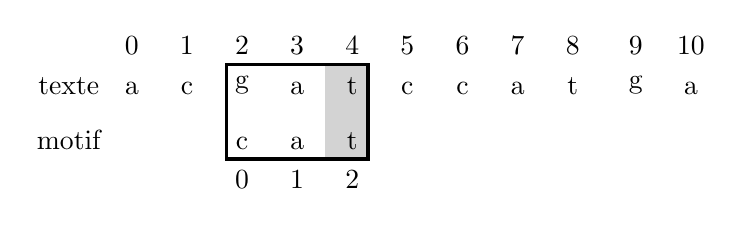
\begin{tikzpicture}
        \fill[LightGray] (4.55,0.5)--(5.1,0.5) -- (5.1,-0.7) -- (4.55,-0.7) -- cycle;
        \foreach \a/\b in {2.1/0,2.8/1,3.5/2,4.2/3,4.9/4,5.6/5,6.3/6,7/7,7.7/8,8.5/9,9.2/10}
            {\node[anchor=south] at (\a,0.5) {\b};}
        \node[anchor=south] at(1.3,0){texte};
        \foreach \a/\b in {2.1/a,2.8/c,3.5/g,4.2/a,4.9/t,5.6/c,6.3/c,7/a,7.7/t,8.5/g,9.2/a}
            {\node[anchor=south] at (\a,0) {\b};}

        \node[anchor=south] at(1.3,-0.7){motif};
        \foreach \a/\b in {3.5/c,4.2/a,4.9/t}
            {\node[anchor=south] at (\a,-0.7) {\b};}
        \foreach \a/\b in {3.5/0,4.2/1,4.9/2}
            {\node[anchor=south] at (\a,-1.2) {\b};}
        \draw[very thick] (3.3,0.5)--(5.1,0.5) -- (5.1,-0.7) -- (3.3,-0.7) -- cycle;
    \end{tikzpicture}
    \captionof{figure}{Comparaison inutile}
    \label{inutile2}
\end{center}
On peut donc directement décaler le motif à l'indice 3 du texte (figure \ref{saut1}).
\begin{center}
    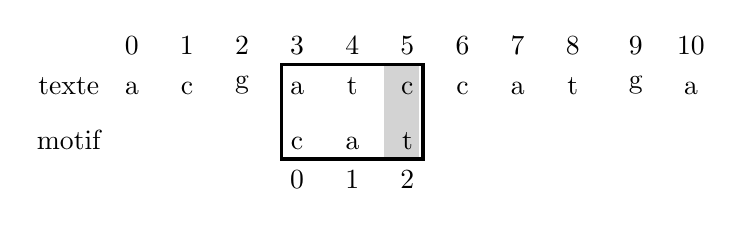
\begin{tikzpicture}
        \fill[LightGray] (5.3,0.5)--(5.75,0.5) -- (5.75,-0.7) -- (5.3,-0.7) -- cycle;
        \foreach \a/\b in {2.1/0,2.8/1,3.5/2,4.2/3,4.9/4,5.6/5,6.3/6,7/7,7.7/8,8.5/9,9.2/10}
            {\node[anchor=south] at (\a,0.5) {\b};}
        \node[anchor=south] at(1.3,0){texte};
        \foreach \a/\b in {2.1/a,2.8/c,3.5/g,4.2/a,4.9/t,5.6/c,6.3/c,7/a,7.7/t,8.5/g,9.2/a}
            {\node[anchor=south] at (\a,0) {\b};}

        \node[anchor=south] at(1.3,-0.7){motif};
        \foreach \a/\b in {4.2/c,4.9/a,5.6/t}
            {\node[anchor=south] at (\a,-0.7) {\b};}
        \foreach \a/\b in {4.2/0,4.9/1,5.6/2}
            {\node[anchor=south] at (\a,-1.2) {\b};}
        \draw[very thick] (4,0.5)--(5.8,0.5) -- (5.8,-0.7) -- (4,-0.7) -- cycle;
    \end{tikzpicture}
    \captionof{figure}{Décalage par saut}
    \label{saut1}
\end{center}
On n'observe pas de correspondance par contre la lettre \textbf{c} existe dans le motif. On va donc le décaler pour les faire coïncider (figure \ref{saut2}).
\begin{center}
    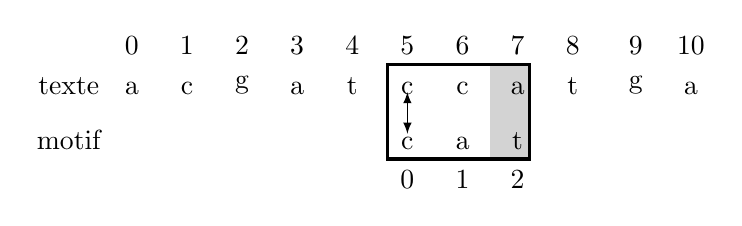
\begin{tikzpicture}
        \fill[LightGray] (6.65,0.5)--(7.15,0.5) -- (7.15,-0.7) -- (6.65,-0.7) -- cycle;
        \foreach \a/\b in {2.1/0,2.8/1,3.5/2,4.2/3,4.9/4,5.6/5,6.3/6,7/7,7.7/8,8.5/9,9.2/10}
            {\node[anchor=south] at (\a,0.5) {\b};}
        \node[anchor=south] at(1.3,0){texte};
        \foreach \a/\b in {2.1/a,2.8/c,3.5/g,4.2/a,4.9/t,5.6/c,6.3/c,7/a,7.7/t,8.5/g,9.2/a}
            {\node[anchor=south] at (\a,0) {\b};}

        \node[anchor=south] at(1.3,-0.7){motif};
        \foreach \a/\b in {5.6/c,6.3/a,7/t}
            {\node[anchor=south] at (\a,-0.7) {\b};}
        \foreach \a/\b in {5.6/0,6.3/1,7/2}
            {\node[anchor=south] at (\a,-1.2) {\b};}
        \draw[very thick] (5.35,0.5)--(7.15,0.5) -- (7.15,-0.7) -- (5.35,-0.7) -- cycle;
        \draw[<->,>=latex] (5.6,-0.38)--(5.6,0.15);
    \end{tikzpicture}
    \captionof{figure}{Décalage par saut}
    \label{saut2}
\end{center}
\begin{aretenir}[]
    On décale la position de recherche dans le texte en fonction de la dernière lettre de la fenêtre.%et de sa présence éventuelle dans le motif
\end{aretenir}
\subsection{Prétraitement du motif}
Pour pouvoir décaler par saut, il faut connaître la dernière position de chaque lettre dans le motif. Le prétraitement consiste à calculer le décalage à appliquer pour amener chaque caractère du motif à la place du dernier caractère.
%exemple figure 8 (lettre c)
% ce prétraitement = coûte un peu mais compensé largement
\begin{aretenir}[Remarque]
    On ne regarde pas la dernière position de la clé (la lettre \emph{t} ici). Sinon la distance associée serait nulle et on resterait sur place après l’avoir lue dans le texte.
    % attention t pourrait être présent ailleurs dans motif $\rightarrow$ on prend en compte alors
\end{aretenir}
\begin{activite}
    Écrire la fonction \textbf{\texttt{pretraitement\_decalages(motif: str) $\rightarrow$ dict}} qui associe chaque lettre du motif (sauf la dernière) à son décalage.
\end{activite}
\subsection{Algorithme de Boyer-Moore (simplifié - version Horspool)}
L'algorithme de Boyer-Moore s'écrit alors:
\begin{center}
\begin{lstlisting}[language=Bash, xleftmargin=2em, xrightmargin=2em]
Créer le tableau des décalages
Tant qu'on n'est pas à la fin du texte
    Comparer le motif à la position du texte
    Si le motif est présent
        Renvoyer la position
    Sinon
        Décaler la fenêtre
Renvoyer -1 si le motif n'est pas présent
\end{lstlisting}
\captionof{code}{Algorithme de Boyer-Moore (version Horspool)}
\label{algo}
\end{center}

\begin{activite}
    \begin{enumerate}
        \item Écrire la fonction \textbf{\texttt{compare(texte: str, position: int, motif: str) $\rightarrow$ bool}} qui renvoie \emph{True} si le motif est présent à la position \emph{i} du texte.
        \item Écrire la fonction \textbf{\texttt{decalage\_fenetre(decalages: dict, taille: int, lettre: str) $\rightarrow$ int}} qui renvoie le décalage à appliquer pour faire coïncider le motif à la dernière \emph{lettre} de la fenêtre. Si la lettre n'est pas présente, la \emph{taille} du motif est renvoyée.
        \item Écrire alors la fonction \textbf{\texttt{boyer\_moore(texte: str, motif: str) $\rightarrow$ int}} qui renvoie la position du motif dans le texte et -1 sinon.
    \end{enumerate}
\end{activite}
% d'autres versions (bad char, good suffix)
\subsection{Complexité}
Intuitivement l'algorithme semble plus rapide que la version naïve car il ne teste pas toutes les lettres du texte.
\begin{center}
    \begin{tabular}{*{15}{c}}
        a&a&a&a&b&a&a&a&a&b&a&a&a&a&b\\
        c&c&c&c&c&&&&&&&&&&\\
    \end{tabular}
    \captionof{figure}{Un cas représentatif}
\end{center}
\begin{activite}
Compter le nombre d'itérations de la recherche avec l'algorithme naïf puis celui de Boyer-Moore.
\end{activite}
\begin{aretenir}[Remarques]
\begin{itemize}
    \item Dans le meilleur des cas, la complexité temporelle de l'algorithme est $O(N/K)$ où N est la taille du texte et N celle du motif.
    \item Plus le motif est long plus l'algorithme est rapide.
\end{itemize}
\end{aretenir}
% O(3.K)
% naïf O(L.K)
\end{document}